\section{Max Flows and Min Cuts}
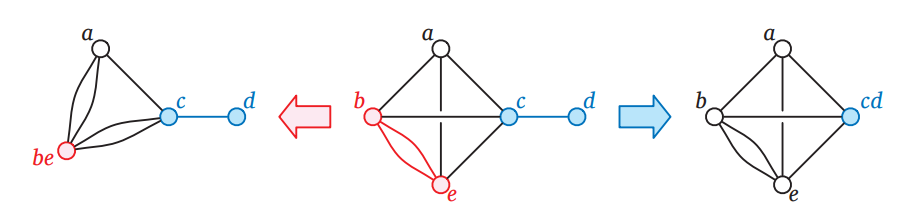
\includegraphics[width=\linewidth]{images/edgecollapse.png}
\subsection{Blind Guess}
\begin{algorithmic}[1]
	\Function{GuessMinCut}{$G$}
		\For{$i \gets n, 2$}
			\State pick a random edge $e$ in $G$
			\State $G \gets G/e$
		\EndFor
		\State \Return the only cut in $G$
	\EndFunction
\end{algorithmic}
$P(n) = \frac{2}{n(n-1)}$

\subsection{Repeated Guessing}
\begin{algorithmic}[1]
	\Function{KargerMinCut}{$G$}
		\State $mink \gets \infty$
		\For{$i \gets 1, N$}
			\State $X \gets \Call{GuessMinCut}{G}$
			\If{$\left|X\right| < mink$}
				\State $mink \gets \left|X\right|$
				\State $minX \gets X$
			\EndIf
		\EndFor
		\State \Return $minX$
	\EndFunction
\end{algorithmic}
Set $N = c \binom{n}{2} \ln n$ for some constant $c$. $P(n) \geq 1 - \frac{1}{n^c}$. \alg{KargerMinCut} computes the min cut of any $n$-node graph with high probability in $O(n^4 \log n)$ time.

\subsection{Not-So-Blindly Guessing}
\begin{algorithmic}[1]
	\Function{Contract}{$G, m$}
		\For{$i \gets n, m$}
			\State pick a random edge $e$ in $G$
			\State $G \gets G/e$
		\EndFor
	\EndFunction
	\Function{BetterGuess}{$G$}
		\If{$G$ has more than 8 vertices}
			\State $G_1 \gets \Call{Contract}{G, n/\sqrt{2} + 1}$
			\State $G_2 \gets \Call{Contract}{G, n/\sqrt{2} + 1}$
			\State $X_1 \gets \Call{BetterGuess}{G_1}$
			\State $X_2 \gets \Call{BetterGuess}{G_2}$
			\State \Return min($X_1, X_2$)
		\Else
			\State use brute force
		\EndIf
	\EndFunction
\end{algorithmic}
$P(n) \geq 1/\log n$. The running time is $O(n^2 \log n)$.

\subsection{Flows}
A \emph{flow} is a function $f$ that satisfies the \emph{conservation constraint} at every vertex $v$: the total flow \emph{into} $v$ is equal to the total flow \emph{out} of $v$.\\

A flow $f$ is \emph{feasible} if $f(e) \leq c(e)$ for each edge $e$. A flow \emph{saturates} edge $e$ if $f(e) = f(c)$, and \emph{avoids} edge $e$ if $f(e) = 0$.

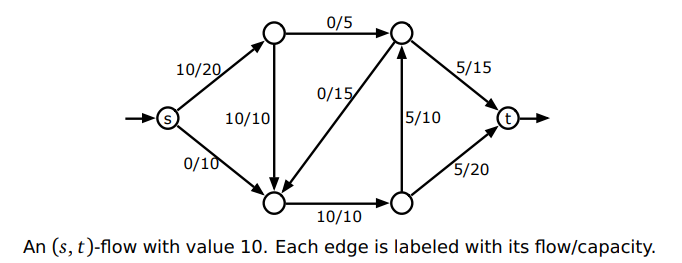
\includegraphics[width=\linewidth]{images/flow.png}

\subsection{Cuts}
A \emph{cut} is a partition of the vertices into disjoint subsets $S$ and $T$ - meaning $S \cup T = V$ and $S \cap T = \emptyset$ - where $s \in S$ and $t \in T$.\\

If we have a capacity function $c$, the \emph{capacity} of a cut is the sum of the capacities of the edges that start in $S$ and end in $T$. The definition is asymmetric; edges that start in $T$ and end in $S$ are unimportant. The \emph{min-cut problem} is to compute a cut whose capacity is as large as possible.

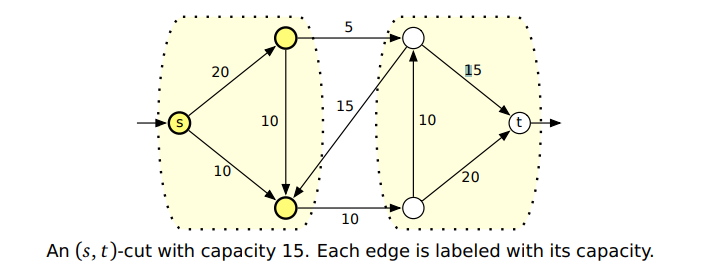
\includegraphics[width=\linewidth]{images/mincut.png}

\begin{theorem}[Maxflow Mincut Theorem]
	In any flow network, the value of the maximum flow is \emph{equal} to the capacity of the minimum cut.
\end{theorem}

\subsection{Residual Capacity}
\[
	c_f(u \rightarrow v) =
	\begin{cases}
		c(u \rightarrow v) - f(u \rightarrow v) & \text{if } u \rightarrow v \in E\\
		f(v \rightarrow u) & \text{if } v \rightarrow u \in E\\
		0 & \text{otherwise}
	\end{cases}
\]

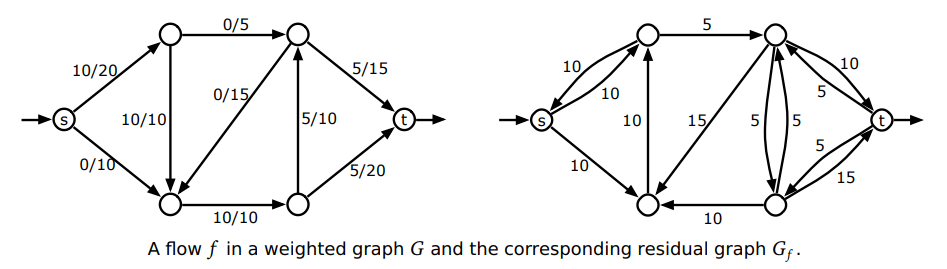
\includegraphics[width=\linewidth]{images/residualgraph.png}

\subsection{Augmenting Paths}
Suppose there is a path $s = v_0 \rightarrow v_1 \rightarrow \cdots \rightarrow v_r$ in the residual graph $G_f$. This is an \emph{augmenting path}. Let $F = \text{min}_i c_f(v_i \rightarrow v_{i+1})$ denote the maximum amount of flow that we can push through the augmenting path in $G_f$. We can augment the flow into a new flow function $f'$:

\[
	f'(u \rightarrow v) =
	\begin{cases}
		f(u \rightarrow v) + F & \text{if } u \rightarrow v \in s\\
		f(u \rightarrow v) - F & \text{if } v \rightarrow u \in s\\
		f(u \rightarrow v) & \text{otherwise}
	\end{cases}
\]

\subsection{Ford-Fulkerson}
Starting with the zero flow, repeatedly augment the flow along \emph{any} path from $s$ to $t$ in the residual graph, until there is no such path.

\subsection{Further Work}
The fastest known maximum flow algorithm, announced by James Orlin in 2012, runs in $O(VE)$ time.